\chapter{FUNDAMENTOS}
\label{sec:fundamentos}


Este é o primeiro capítulo da parte central do trabalho, isto é, o desenvolvimento, a parte mais extensa de todo o trabalho. Geralmente o desenvolvimento é dividido em capítulos, cada um com seções e subseções, cujo tamanho e número de divisões variam em função da natureza do conteúdo do trabalho.

Em geral, a parte de desenvolvimento é subdividida em três capítulos:

\begin{itemize}
    \item \textit{referencial ou embasamento teórico} – texto no qual se deve apresentar os aspectos teóricos, isto é, os conceitos utilizados e a definição dos mesmos; nesta parte faz-se a revisão de literatura sobre o assunto, resumindo-se os resultados de estudos feitos por outros autores, cujas obras citadas e consultadas devem constar nas referências;

    \item \textit{metodologia do trabalho ou procedimentos metodológicos} – deve constar o instrumental, os métodos e as técnicas aplicados para a elaboração do trabalho;

    \item \textit{resultados} – devem ser apresentados, de forma objetiva, precisa e clara, tanto os resultados positivos quanto os negativos que foram obtidos com o desenvolvimento do trabalho, sendo feita uma discussão que consiste na avaliação circunstanciada, na qual se estabelecem relações, deduções e generalizações.

\end{itemize}

É recomendável que o número total de páginas referente à parte de desenvolvimento não ultrapasse 60 (sessenta) páginas.

\section{Como Adicionar IMAGENS}

    Para adicionar uma imagem você deverá seguir o seguinte padrão.

\begin{lstlisting}[language=TeX, caption{Código da Imagem da Logo}, label{cod:logoIFPA}]
\begin{figure}[H]
    \setstretch{1.5}\centering\footnotesize
    \caption{Logo do IFPA}
    \begin{center}
        
\includegraphics[width=0.3\textwidth]{ifpa-logo.png}
    \end{center}
    \label{fig:logoIFPA}
    \par Fonte: Google Imagens
\end{figure}
\end{lstlisting}

\hfill

\begin{figure}[H]
    \setstretch{1.5}\centering\footnotesize
    \caption{Logo do IFPA}
    \begin{center}
        
\includegraphics[width=0.3\textwidth]{ifpa-logo.png}
    \end{center}
    \label{fig:logoIFPA}
    \par Fonte: Google Imagens
\end{figure}


\begin{lstlisting}[language=TeX, caption=Codigo da Imagem do Brasao]
\begin{figure}[H]
    \setstretch{1.5}\centering\footnotesize
    \caption{Brasão do Brasil}
    \begin{center}
        
\includegraphics[width=0.5\textwidth]{DeusAcimaDeTodos.png}
    \end{center}
    \label{fig:brasaoBrasil}
    \par Fonte: Google Imagens
\end{figure}
\end{lstlisting}

\hfill

\begin{figure}[H]
    \setstretch{1.5}\centering\footnotesize
    \caption{Brasão do Brasil}
    \begin{center}
        
\includegraphics[width=0.5\textwidth]{DeusAcimaDeTodos.png}
    \end{center}
    \label{fig:brasaoBrasil}
    \par Fonte: Google Imagens
\end{figure}

\begin{lstlisting}[language=TeX, caption=Codigo da Imagem do Album]
\begin{figure}[H]
    \setstretch{1.5}\centering\footnotesize
    \caption{Álbum A Presença da Glória da banda Santa Geração}
    \begin{center}
        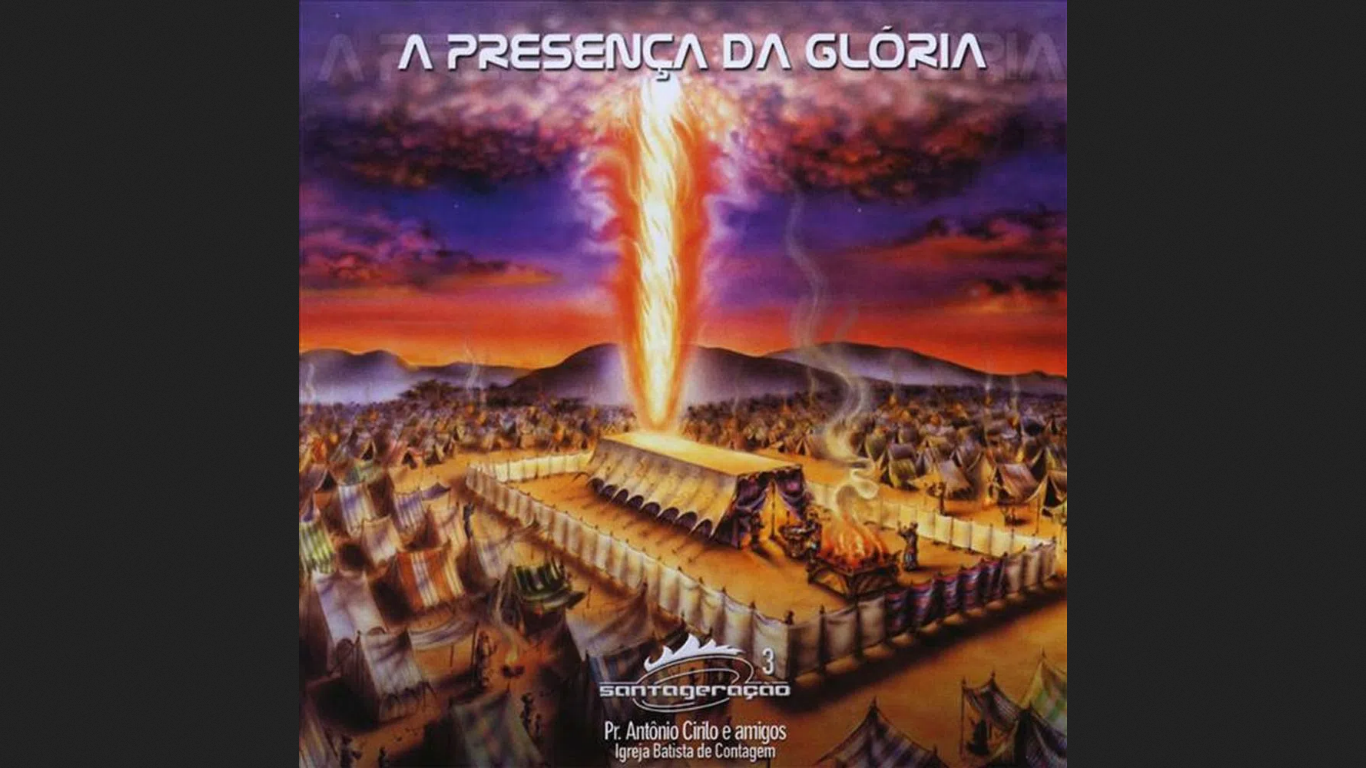
\includegraphics[width=0.5\textwidth]{presencaDaGloria.png}
    \end{center}
    \label{fig:capaPresencaDaGloria}
    \par Fonte: Google Imagens
\end{figure}
\end{lstlisting}

\begin{figure}[H]
    \setstretch{1.5}\centering\footnotesize
    \caption{Álbum A Presença da Glória da banda Santa Geração}
    \begin{center}
        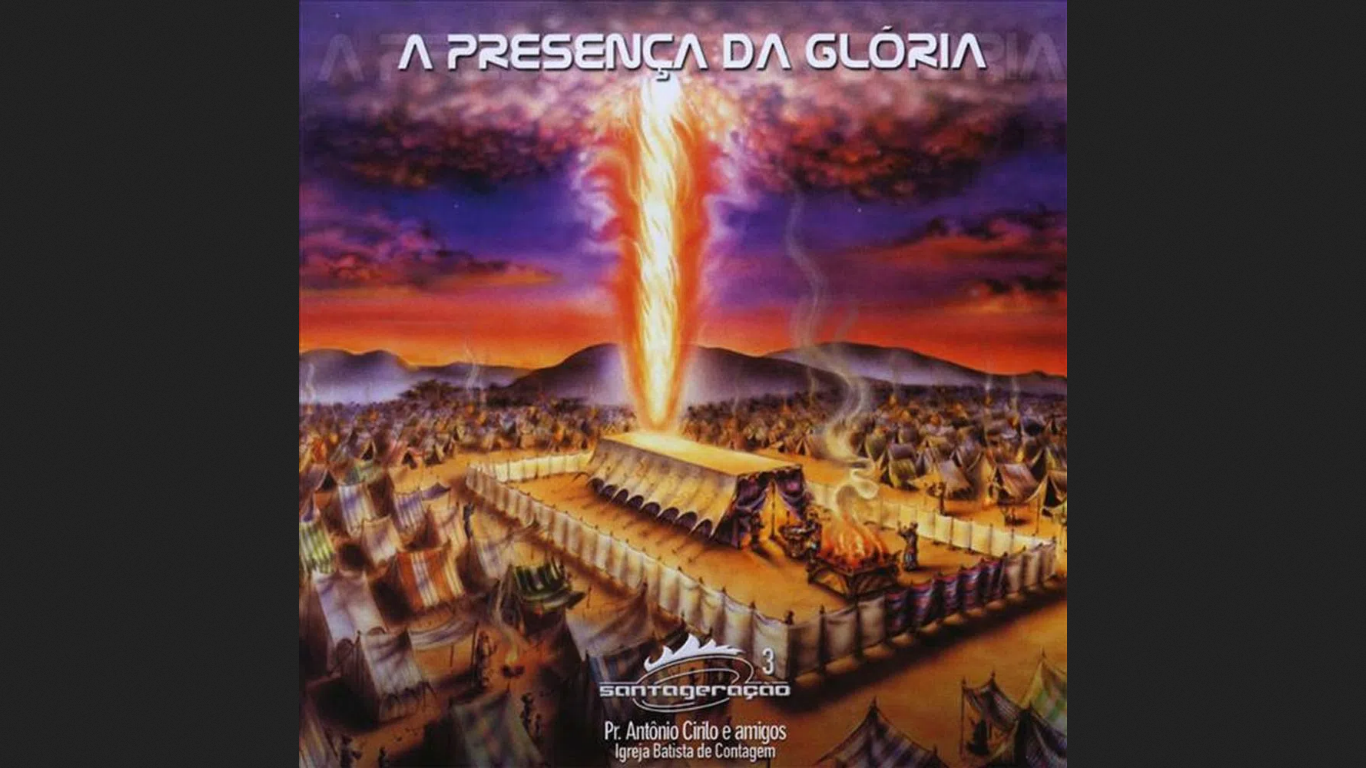
\includegraphics[width=0.5\textwidth]{presencaDaGloria.png}
    \end{center}
    \label{fig:capaPresencaDaGloria}
    \par Fonte: Google Imagens
\end{figure}
		
\section{Dando Nome e Referenciando Figuras no Texto}
	
Referenciamento da figura inserida na seção anterior: ~\autoref{fig:logoIFPA}.

\hfill

Comando:

\textbackslash ref\{fig:logoIFPA\}

\hfill

Esse referenciamento é possível devido ao padrão de inserção de imagem sugerido neste documento, o qual um dos campos da imagem é o \textbackslash capition acompanhado do \textbackslash label , onde definimos como poderemos referenciar tal imagem no decorrer do texto.

\hfill

\textbackslash label\{ fig:NomeDaFigura \}

\hfill

No campo \"NomeDaFigura\" podemos definir como iremos referenciar tal imagem no decorrer do texto usando o comando \textbackslash ref\{ fig:NomeDaFigura \}

\section{Abreviaturas e Simbolos}

Para utilizar abreviaturas e simbolos, basta utilizar o comando barra $\backslash$ combinado com ac ou acl.

Dentro das chaves você deve adicionar a palavra-chave da abreviatura ou símbolo

$\backslash$ac \{ \}

$\backslash$acl \{ \}

\hfill

Exemplo:

$\backslash$ac \{ abntex \}

AC \ac{abntex}.

$\backslash$acl \{ abntex \}

ACL \acl{abntex}.

\hfill

Simbolos e a versão por extenso.

$\backslash$ac \{ megaByte \}

\ac{megaByte}

$\backslash$acl \{ megaByte \}

\acl{megaByte}

\hfill

$\backslash$ac \{ lambda \}

AC \ac{lambda}.

$\backslash$acl \{ lambda \}

ACL \acl{lambda}.


\section{Glossário}

Para fazer uso do glossário (um elemento pós-textual), você deve usar o arquivo "glossário.tex" presente na pasta "Escritor", e seguir o exemplo que lá consta para adicionar as SUAS palavras que deverão constar no glossário.

No decorrer do texto você deverá usar o padrão \gls{fórmula} para marcar as palavras no momento conveniente do texto em que estas deverão aparecer.

Com isso, somente as palavras que você marcou usando o comando \textbackslash gls\{\} irão aparecer.

\textbackslash gls\{ sample \}

\gls{sample}.

\hfill

\textbackslash gls\{ fórmula \}

\gls{fórmula}.